%%%%%%%%%%%%%%%%%%%%%%%%%%%%%%%%%%%%%%%%%%%%%%%%%%%%%%%%%%%%%%%%%%%%%%%%%%%%%%%%
%2345678901234567890123456789012345678901234567890123456789012345678901234567890
%        1         2         3         4         5         6         7         8

%\documentclass[letterpaper, 10 pt, conference]{ieeeconf}  % Comment this line out
                                                          % if you need a4paper
\documentclass[a4paper, 10pt, conference]{ieeeconf}      % Use this line for a4
                                                          % paper

\IEEEoverridecommandlockouts                              % This command is only
                                                          % needed if you want to
                                                          % use the \thanks command
\overrideIEEEmargins
% See the \addtolength command later in the file to balance the column lengths
% on the last page of the document


\let\labelindent\relax

% The following packages can be found on http:\\www.ctan.org
\usepackage{graphics} % for pdf, bitmapped graphics files
\usepackage{epsfig} % for postscript graphics files
%\usepackage{mathptmx} % assumes new font selection scheme installed
%\usepackage{times} % assumes new font selection scheme installed
\usepackage{amsmath} % assumes amsmath package installed
\usepackage{amssymb}  % assumes amsmath package installed
\let\proof\relax
\let\endproof\relax
\usepackage{amsthm}

\usepackage{url}
\usepackage[ruled, vlined, linesnumbered]{algorithm2e}
%\usepackage{algorithm}
\usepackage{verbatim} 
%\usepackage[noend]{algpseudocode}
\usepackage{soul, color}
\usepackage{lmodern}
\usepackage{fancyhdr}
\usepackage[utf8]{inputenc}
\usepackage{fourier} 
\usepackage{array}
\usepackage{makecell}
\usepackage[inline]{enumitem}
\usepackage{url}
\usepackage{subcaption} 
\usepackage{hyperref}
\usepackage{dblfloatfix}
\usepackage[british]{babel}
\usepackage[sorting=none, style=ieee, bibstyle=ieee, backend=biber, citestyle=numeric-comp]{biblatex}
\addbibresource{reference.bib}



\theoremstyle{plain}
\newtheorem{thm}{Theorem}[section] % reset theorem numbering for each chapter
\theoremstyle{definition}
\newtheorem{nota}[thm]{Notation}
\newtheorem{defn}[thm]{Definition} % definition numbers are dependent on theorem numbers
\newtheorem{exmp}[thm]{Example} % same for example numbers
\newtheorem{hyp}{Hypothesis}



\SetNlSty{large}{}{:}

\renewcommand\theadalign{bc}
\renewcommand\theadfont{\bfseries}
\renewcommand\theadgape{\Gape[4pt]}
\renewcommand\cellgape{\Gape[4pt]}

\newcommand{\rework}[1]{\todo[color=yellow,inline]{#1}}

\makeatletter
\newcommand{\rom}[1]{\romannumeral #1}
\newcommand{\Rom}[1]{\expandafter\@slowromancap\romannumeral #1@}
\makeatother

\pagestyle{plain} 

\title{\LARGE \bf
Dynamische Windows processing in RDF Mapping engines voor data streams 
}

%\author{ \parbox{3 in}{\centering Huibert Kwakernaak*
%         \thanks{*Use the $\backslash$thanks command to put information here}\\
%         Faculty of Electrical Engineering, Mathematics and Computer Science\\
%         University of Twente\\
%         7500 AE Enschede, The Netherlands\\
%         {\tt\small h.kwakernaak@autsubmit.com}}
%         \hspace*{ 0.5 in}
%         \parbox{3 in}{ \centering Pradeep Misra**
%         \thanks{**The footnote marks may be inserted manually}\\
%        Department of Electrical Engineering \\
%         Wright State University\\
%         Dayton, OH 45435, USA\\
%         {\tt\small pmisra@cs.wright.edu}}
%}

\author{Sitt Min Oo
\\
\\
Promotoren: Prof.~Dr. Ruben Verborgh and Dr. Anastasia Dimou\\
Begeleider: Gerald Haesendonck
}


\begin{document}



\maketitle
\thispagestyle{plain}
\pagestyle{plain}



%%%%%%%%%%%%%%%%%%%%%%%%%%%%%%%%%%%%%%%%%%%%%%%%%%%%%%%%%%%%%%%%%%%%%%%%%%%%%%%%
%%%%%%%%%%%%%%%%%%%%%%%%%%%%%%%%%%%%%%%%%%%%%%%%%%%%%%%%%%%%%%%%%%%%%%%%%%%%%%%%
\begin{abstract}

De huidige state-of-the-art benaderingen voor het mappen van niet-RDF naar RDF data in 
een streaming omgeving richten zich meer op de efficiëntie van het 
mapping proces met minimale ondersteuning voor multi-stream verwerking. 
De bestaande benaderingen voor de ondersteuning van eenvoudige multi-stream 
processing operatoren in mapping engines zijn zeer beperkt of passen een vaste window grootte toe.

Daarom hebben we in RMLStreamer een dynamisch venstermechanisme geïmplementeerd, dat 
de grootte aanpast aan de veranderende kenmerken van de stroom met
verwaarloosbare geheugenoverhead, lage latentie en hoge doorvoer. We evalueerden het dynamische venster
onder verschillende werkbelastingen met variërende streamsnelheid. De resultaten 
tonen aan dat het een latentie bereikt in het milliseconden bereik, met een hogere 
doorvoer dan vensters met een vaste grootte in alle werklast situaties. \\ 
\end{abstract}

\begin{keywords}
RDF, RMLStreamer, RML, Adaptieve vensters, Dynamische vensters,
Stream joins, Multi-stream verwerking.

\end{keywords}

%%%%%%%%%%%%%%%%%%%%%%%%%%%%%%%%%%%%%%%%%%%%%%%%%%%%%%%%%%%%%%%%%%%%%%%%%%%%%%%%
%%%%%%%%%%%%%%%%%%%%%%%%%%%%%%%%%%%%%%%%%%%%%%%%%%%%%%%%%%%%%%%%%%%%%%%%%%%%%%%%
\section{INTRODUCTIE}
\label{chap:intro}

Diverse gegevensformaten, zoals CSV of HTML, zijn niet ontworpen om de semantiek van hun gegevens te bevatten
waardoor machines deze gegevens niet automatisch kunnen interpreteren. 
Om ervoor te zorgen dat deze heterogene gegevensformaten interpreteerbaar en 
verwerkbaar zijn door machines, zijn gegevensformaten gebaseerd op W3C-normen, zoals Resource Description 
Framework (RDF) triples~\cite{intro_rdf}, worden ontwikkeld. 
Er bestaan state-of-the-art benaderingen om heterogene data te consolideren
en deze te transformeren naar een RDF serialisatie in een streaming omgeving. 

Deze benaderingen ondersteunen traditionele stream operatoren zoals joins en aggregaties. 
Echter, ze houden geen rekening met
de karakteristieken van streaming data bronnen zoals snelheid en 
tijd-correlaties tussen de verschillende
invoerstromen, hetzij als gevolg van de 
vaste grootte van vensters of aangepaste oplossingen die zij toepassen. 

Daarom stellen wij een dynamisch venster voor als oplossing voor de variërende kenmerken van streaming data. Wij evalueerden onze 
benadering met de join operator toegepast binnen het venster. 
Het dynamische venster verbetert de prestaties van de 
join operator met hogere doorvoer, lagere latency en 
vergelijkbaar geheugengebruik vergeleken met een venster met vaste grootte.

De broncode en de code voor de evaluatieopstelling zijn te vinden op
\url{https://github.com/RMLio/RMLStreamer/tree/feature/window_joins}, en 

respectievelijk \href{https://github.com/Kortika/Thesis-test-scripts.git}{https://github.com/Kortika/Thesis-test-scripts.git}.


\section{RELATED WORKS} 
\label{sec:RELATED WORKS} 
There exists state-of-the-arts approaches to map non-RDF data 
to RDF data in a streaming environment. These approaches 
implement diferent strategies when it comes to applying 
multi-stream processing. Furthermore, we will also outline
the existing works on windowing to handle changing characteristics 
of the input data stream. 

\subsection{Mapping implementations}
\subsubsection{SPARQL-Generate} 
SPARQL-Generate~\cite{sparql_generate} 
is based on an extension of SPARQL 1.1 query language, to leverage 
its expressiveness and extensibility. 
It can be implemented on top 
of any existing SPARQL query engine. 
M. Lefran\c{c}ois~\cite{sparql_generate} clarified that when joining
records from two different streams, SPARQL-Generate will fully consume the records 
from the "parent" stream and index it internally in memory first, before 
iteratively consuming the "child" stream for joining. 

\subsubsection{TripleWave} 
TriplWave~\cite{triple_wave}  is based on an extension of 
R2RML to consume heterogeneous data for publication of RDF data. 
Therefore, it only focuses on the mapping of non-RDF data stream to RDF data stream. 
Although it supports simple \emph{join} operator, it does not have a 
dynamic window to handle changing characterisitcs of a data stream.

\subsubsection{RDFGen}
RDF-Gen~\cite{rdf_gen} is based on its own custom syntax 
similar to a combination SPARQL and Turtle syntax. It processes the input 
individually therefore it employs windowing to perform multi stream operator. 
However, since the implementation is closed source, we could not confirm if 
the window is fixed size or dynamic. 

\subsubsection{RMLStreamer}
RMLStreamer~\cite{rml_streamer}
was developed to parallelize the ingestion and mapping process of RDF data generation pipeline. 
It is based on the work of RMLMapper~\cite{rml}, an RDF mapping engine consuming bounded data and mapping them to RDF data with the use of RML. Hence, RMLStreamer can also 
process heterogeneous data and generate RDF data. It does not support 
multi stream operator at this moment, however, the ease of scalability by RMLStreamer
is desirable as a stream mapping engine. 


\subsection{Windows}
Several studies have been conducted to 
improve the join algorithms in windows~\cite{vctw_join, join_tracking, grubjoin, approximate_window_sem, approx_window}. 
The approaches in ~\cite{grubjoin, approximate_window_sem, approx_window} are based 
on dropping some of the records to be joined through \emph{load shedding} if the 
records failed to meet a threshold. These threshold calculation requries 
memory overhead for storing statistical model per window or 
assumption of the stream being in-order for them to work
~\cite{grubjoin, approximate_window_sem, approx_window}.

On the other hand, VC-TWJoin~\cite{vctw_join} considers only the velocity of the 
stream to adjust the window sizes. 
However, the approach is unstable when the data stream has periodic bursts of data.
It either increases or decreases the size of the window when themetric triggers 
the threshold of the algorithm. In the worst-case scenario it 
can lead to cyclic increase and 
decrease of window sizes if the metric borders around the threshold with every 
update of the metric.







\section{DYNAMISCH VENSTER}%
\label{sec:Dynamic Window}
Een dynamisch venster is een type gepartitioneerd venster~\cite{generic_window_sem}.
Wij definiëren het als een groep subvensters, die hun grootte dynamisch aanpassen volgens de kenmerken 
van de gegevensstroom. Het groepeert de binnenkomende stromen eerst in verschillende partities, volgens 
de \emph{key} attribuutwaarde van de records. Vervolgens worden deze gegroepeerde records toegewezen 
aan individuele subvensters. Deze subvensters passen hun eigen grootte onafhankelijk van elkaar aan 
bij elke update-cyclus. Bovendien zullen de subvensters onafhankelijk van elkaar zijn, zodat 
dat de stroomsnelheid lokaal is voor de attribuutwaarde waarvoor elk subvenster verantwoordelijk is. 

\subsection{Dynamische vensterverbinding}
\label{sub:Dynamic window join}

Het gebruikte join-algoritme is een variant van Symmetric Hash Join~\cite{symmetric_hash_join}. 
De subvensters zelf werken als een hashtabel, die records bevat met een 
specifieke \emph{sleutel} --- aangezien ze \emph{gepartitioneerd} zijn. 
De records worden samengevoegd door de relevante stroom af te tasten en het 
resultaat te genereren. 


\subsection{Dynamisch venster-algoritme}%
\label{sub:Dynamic window algorithm}
Voor elk subvenster worden de volgende configuratieparameters 
voorzien: 

\begin{itemize}
    \item $\Delta n$: het \textbf{initiële} tijdsinterval voor de volgende ontruimingstrigger. 
    \item $\epsilon_u$: de bovengrensdrempel voor de totale kosten metriek.
    \item $\epsilon_l$: de ondergrens voor de totale-kostenmethode. 
    \item $U$: de bovengrens voor de venstergrootte. 
    \item $L$: de ondergrens voor de venstergrootte. 
\end{itemize}

Aangezien wij de join operator implementeren, wordt de trigger-event afgevuurd wanneer de huidige record 
$r_c$ binnenkomt, en de symmetrische hash join wordt uitgevoerd. We duiden het huidige venster aan als 
$W$ met de grootte als $|W|$. De stromen worden aangeduid als $S_P$ en $S_C$ met 
de overeenkomstige toestanden $List_P$ en $List_C$, voor respectievelijk de ouder- en 
de kindstroom. De toestanden bevatten de records van hun 
respectievelijke streams in de subvensters.

De ontruimingstrigger wordt afgevuurd telkens wanneer het huidige watermerk 
$w \ge |W| + \Delta n$. Bij elke ontruimingstrigger berekenen we
de kosten voor elke staat van €71$List_P$ en $List_C$, die de records van $S_P$ en $S_C$ bevatten
respectievelijk. De kosten voor €17 €, idem voor €18 €. 
De totale kosten bedragen $m = cost(List_P) + cost(List_C)$ en worden getoetst aan de drempels $\epsilon_l$ en $\epsilon_u$. Indien $\epsilon_l \le m \le \epsilon_u$, 
$\Delta n$ blijft het gelijk, anders wordt het dienovereenkomstig aangepast. Dit zorgt voor enige stabiliteit 
in de venstergrootte door dezelfde grootte te behouden als de kosten binnen de drempels liggen. 
Hoe hoger $m$, hoe hoger de stroomsnelheid. Het subvenster moet dus vaak worden 
worden uitgezet en $\Delta n$ worden verlaagd om het geheugengebruik te verminderen. Er is ook een limiet op de 
minimum en maximum venstergrootte, respectievelijk $L$ en $U$, om ervoor te zorgen dat de venstergrootte 
grootte $\Delta n$ niet oneindig in grootte blijft groeien of krimpen in een worst-casescenario. 
De grootte van de lijsttoestanden 
worden ook geactualiseerd overeenkomstig $Size(List_P) = Size(List_P) * cost(List_P) + 0.5$.
Hetzelfde geldt voor €30. 
Het dynamische venster handhaaft dus een 
ideale grootte door $\Delta n, Size(List_P)$ en $Size(List_C)$ aan te passen aan 
de stroomsnelheid. De pseudocode voor het uitzettingsalgoritme wordt gepresenteerd in Algoritme~\ref{alg:dynamic_eviction}.

Dit algoritme voor het dynamische venster is een aanpassing van VC-TWindow~\cite{vctw_join} met 
verbeteringen voor stabiliteit in de venstergrootte, duidelijkheid in de voor updates gebruikte metriek, en lokalisatie 
van de bijwerking van de venstergrootte voor elk subvenster.  

\begin{algorithm}[htbp]
    \DontPrintSemicolon
    \KwData{$\Delta n, \epsilon_u, \epsilon_l, U, L, List_P, List_C, S_P, S_C$}

    $cost(List_P) = |S_P| / Size(List_P)$      
    
    $cost(List_C) = |S_C| / Size(List_C)$     


    totale kosten $ m = cost(List_P) + cost(List_C)$  
  
    \If{$m > \epsilon_u$} 
    {
    
        $\Delta n = \Delta n / 2 $ 
        
        $Size(List_P) = Size(List_P) * (cost(List_P) + 0.5)$  

        $Size(List_C) = Size(List_C) * (cost(List_C) + 0.5)$  
    }
    \ElseIf{$m < \epsilon_l$}
    {
   
        $\Delta n = \Delta n * 2$ 

        $Size(List_P) = Size(List_P) * (cost(List_P) + 0.5)$  

        $Size(List_C) = Size(List_C) * (cost(List_C) + 0.5)$  
    }

    beide schoonmaken $List_C \text{ and } List_P$
    \caption{Dynamisch raam $onEviction$ routine}
    \label{alg:dynamic_eviction}
\end{algorithm}




\section{IMPLEMENTATIE}%
\label{sec:Implementation}

Het dynamische venster is ge\"implementeerd voor RMLStreamer 
om de mogelijkheden ervan uit te breiden voor eenvoudige streamverwerking door 
meerdere streams samen te voegen.  Bovendien hebben we RML uitgebreid
uitgebreid met nieuwe ontologieën om de configuratie van het venster mogelijk te maken. 

\subsection{RML ontologie-uitbreiding}
We hebben RML uitgebreid met ondersteuning voor de configuratie van het venster wanneer
het samenvoegen van de \emph{reference object map} met zijn \emph{parent triples map}. 
Momenteel ondersteunt het alleen de rudimentaire 
configuratie van het type verbinding dat moet worden toegepast.

\subsection{Dynamisch venster}
Het dynamische venster is ge\"implementeerd met behulp van Apache Flink's 
\emph{KeyedCoProcessFunction} API met het statusbeheer 
gedaan met behulp van Flink's \emph{ListStates}.

\section{EVALUATIE}
\label{chap:Evaluation}

Om de doeltreffendheid te meten van dynamische windowing voor multi-stream operatoren tijdens de 
mapping van niet-RDF heterogene gegevens moeten we de volgende 
metrieken van ons stream processing framework: \emph{CPU gebruik}, \emph{latency}, \emph{doorvoer},
\emph{geheugengebruik}, en \emph{compleetheid}. 

\subsection{Gegevens}
We gebruiken dezelfde gegevens 
als de benchmark in het artikel van Van Dongen en Van den Poel~\cite{evalution_of_spe}. 
De gegevens zijn afkomstig van de NDW (Nationale Databank Wegverkeersgegevens) uit 
Nederland~\footnote{NDW-datasite: \href{http://opendata.ndw.nu/}{http://opendata.ndw.nu/} }.
Het bestaat uit metingen van het aantal auto's en hun gemiddelde snelheid over de verschillende 
rijstroken op een snelweg. 
De sensorgegevens werden door een Kafka-publisher naar twee topics doorgespeeld, namelijk 
\emph{ndwflow} en \emph{ndwspeed}, voor respectievelijk het aantal auto's en de gemiddelde snelheid.

\subsection{Evaluatie setup}

Docker\footnote{Docker: \url{https://www.docker.com}} is 
opgezet met de containers 
zoals ge\"illustreerd in figuur~\ref{fig:docker_setup}. De docker-containers 
draaien op een standalone machine om de invloed van 
netwerkcommunicatie zo veel mogelijk te beperken. Apache Kafka wordt gebruikt 
als de berichtenmakelaar voor onze gegevens. De setup voor de Kafka broker is 
hetzelfde als beschreven in \cite{evalution_of_spe}. 



\begin{figure}[htpb]
    \centering
    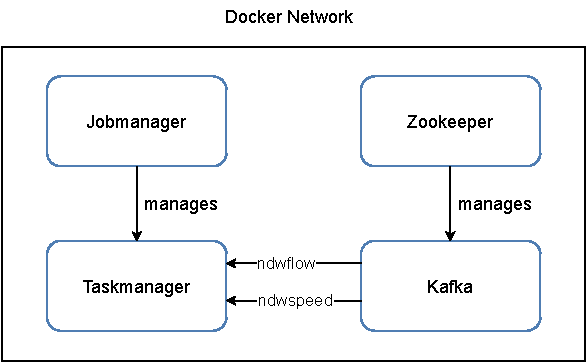
\includegraphics[width=\columnwidth]{fig/docker_setup.pdf}
    \caption[Setup of application containers inside the same docker network.]{ 
Setup van applicatiecontainers binnen hetzelfde docker netwerk.
De kafka topics \emph{ndwflow} en \emph{ndwspeed} worden verbruikt door de 
RMLStreamer job binnen de Taskmanager.}
    \label{fig:docker_setup}
\end{figure}

\subsection{Metingen}%
\label{sub:Metrics measurement}

CPU-gebruik, doorvoer, geheugen, en latency blootgesteld 
door Flink's Rest API, worden constant elke 100ms opgevraagd door een 
Python script scraper.
CPU gebruik, doorvoer 
en geheugengebruik worden intern gemeten door Flink,
terwijl latency meting 
handmatig wordt ge\"implementeerd met behulp van Flink's Metrics API om nauwkeuriger de hoeveelheid tijd te meten 
tijd die een record in het venster doorbrengt voordat het verwerkt wordt. 

De bovengenoemde metrieken worden gemiddeld over de geparallelliseerde window operators.
Intersection over union (IOU) wordt gebruikt als de metriek om de volledigheid te meten
van het samengevoegde resultaat dat door de vensters wordt gegenereerd.  


\subsubsection{CPU-gebruik}%
\label{ssub:CPU usage}
Voor CPU-gebruik meten we het CPU-gebruik van Taskmanager, aangezien die 
verantwoordelijk is voor het uitvoeren van de RMLStreamer-code. 

\subsubsection{Doorvoer}%
\label{ssub:Throughput}
De doorvoermeting wordt gedefinieerd als het aantal records dat per seconde door de 
vensteroperator per seconde. 
Deze wordt gemeten aan de uitvoer van de window operator, aangezien we de 
uitvoerprestaties van de windowoperators willen meten. 


\subsubsection{Geheugengebruik}%
\label{ssub:Memory usage}
Vanwege de beperking in granulariteit van metingen in Flink, 
JVM heap geheugen van de job gebruikt om het geheugengebruik van de window 
operator. We verwachten dat het geheugengebruik door andere operators in de job 
consistent en laag is over de verschillende evaluatieruns, omdat het stateless operators zijn.

\subsubsection{Latency meting}%
\label{ssub:Latency measurement}
We meten de latentie door een tijdstempel toe te voegen aan de 
records voordat ze het venster binnenkomen. 
Zodra de records verwerkt zijn en na de join worden uitgezonden, wordt het verschil 
tussen de huidige verwerkingstijd en de bijgevoegde oude verwerkingstijd 
genomen als de \emph{latency} voor de records. 

\subsubsection{Voltooidheidsmeting}%
\label{ssub:Completeness measurement}
Om \emph{begrensde} invoergegevens te genereren voor 
de static mapping engine, schrijven we de opgeslagen gegevens van de topics 
in een bestand op schijf. Deze invoergegevens worden door RMLStreamer verwerkt in de modus voor 
verwerkingsmodus om de \emph{complete} set triples te genereren. 

De gegenereerde output triples van de evaluatie van de vensters en de verwerking van de begrensde gegevens worden 
gebruikt om de IOU-metriek te berekenen om de gelijkenis tussen de twee outputs te meten.    



\subsection{Werklastscenario's}
\label{sec:workload}
We evalueren onze dynamische vensterimplementatie onder verschillende werklastscenario's. 
Deze werklasten zijn vergelijkbaar met die welke in~\cite{evalution_of_spe} zijn gebruikt, voor zover relevant.

\subsubsection{Werklast voor latentiemeting}
Meting van de \emph{latency} die alleen wordt veroorzaakt 
door de vensterimplementaties, vereist dat het stroomverwerkingsraamwerk niet wordt 
door aanzienlijke \emph{doorvoer} wordt belast. Dus, de Kafka makelaar 
de records op een zeer lage constante snelheid van ongeveer 400 berichten per seconde voor 
deze werklast.
We noemen dit in de paper \emph{constant} stream rate. 

\subsubsection{Werklast met periodieke burst}
We evalueren onze implementatie op zijn vermogen om te gaan met onstabiele 
streaming gegevensbronnen met variërende snelheid.
De werklast heeft een constante lage streamsnelheid met af en toe een 
uitbarsting van gegevens. Daarom worden elke 10 seconden 38 000 records gepubliceerd, wat 
ongeveer 170 tot 180 ms duurt, aangezien de tijd die nodig is om te publiceren kan afwijken op basis van de 
last van de Kafka-brokers.
We duiden dit in de paper aan als \emph{periodic} stream rate. 

\subsubsection{Werklast voor de volledigheid}
We zullen twee stream rates gebruiken, constant en periodiek, 
om de \emph{compleetheid} te meten van de resultaten gegenereerd 
door de verschillende vensters.







\section{RESULTATEN EN DISCUSSIE}%
\label{chap:Results and Discussion}

De evaluaties van de werklasten zijn meerdere keren uitgevoerd om de resultaten consistent te houden. 
Voor elke werklast geven we een kort overzicht van de prestatiewinst 
die door het Dynamische window wordt bereikt. 

\subsection{Werklast voor latentiemeting}%
\label{sec:Results Workload for latency measurement}
Voor latency heeft Tumbling venster een mediane waarde van 1915ms, 
met latentie vari\"erend van 1081ms tot 2624ms (Figuur~\ref{fig:constant_tumb_boxplot})
meer dan $10\times$ de latentie van Dynamisch venster, dat een mediaan heeft 
van 57 en vari\"erend van 39 tot 120ms (Figuur ~\ref{fig:constant_dynamic_boxplot}). 
Onze verbetering om de \emph{trigger} gebeurtenis af te vuren telkens wanneer een
nieuw record arriveert in het 
subvenster, maakt het mogelijk 
Dynamisch venster een latentie van minder dan een seconde bereiken. 

Dynamisch venster heeft een 
gestage doorvoer van ongeveer 17200 records per seconde terwijl Tumbling venster schommelt tussen 
12500 en 12800 records per seconde alvorens zich te stabiliseren op 12750 records per seconde (figuur~\ref{fig:constant_thorughput}). 
Dit is het gevolg van de aanpassing van de venstergrootte op subvensterniveau, waardoor Dynamisch venster op meer records kan wachten 
met onregelmatige \emph{key} attributen in de stroom, alvorens het subvenster uit te zetten. 
Tumbling venster daarentegen 
verwijdert altijd de inhoud van het venster na 2 seconden zonder te wachten op meer 
records.

Het relatieve geheugengebruik van Dynamisch venster vergeleken met Tuimelend venster 
is vergelijkbaar gedurende de levensduur van de 
evaluatierun (figuur ~\ref{fig:constant_mem_diff}). 
Dynamisch venster veroorzaakt onregelmatige \emph{pieken} in geheugengebruik van meer dan
100 MB meer dan Tumbling venster op een bepaald punt in de evaluatieduur. 
Dit kan worden toegeschreven 
aan de subvensters van Dynamisch venster die groter worden als gevolg van de lage stream 
snelheid. Echter,
Dynamisch venster stabiliseert zich op een meer optimale 
venstergrootte, waar het minder geheugen gebruikt dan Tumbling vensters. 
In het slechtste geval gebruikt het net zoveel geheugen als Tumbling venster gedurende de evaluatie. 

Het CPU-gebruik is ongeveer 7\%
hoger voor Dynamisch venster, omdat extra verwerking van de berekening van de metriek nodig is en 
de doorvoer stijgt tegelijkertijd, waardoor RMLStreamer meer samengevoegde records moet verwerken.
(Figuur ~\ref{fig:constant_cpu}). 

\begin{figure}[htbp]
    \begin{subfigure}[b]{0.5\columnwidth}
        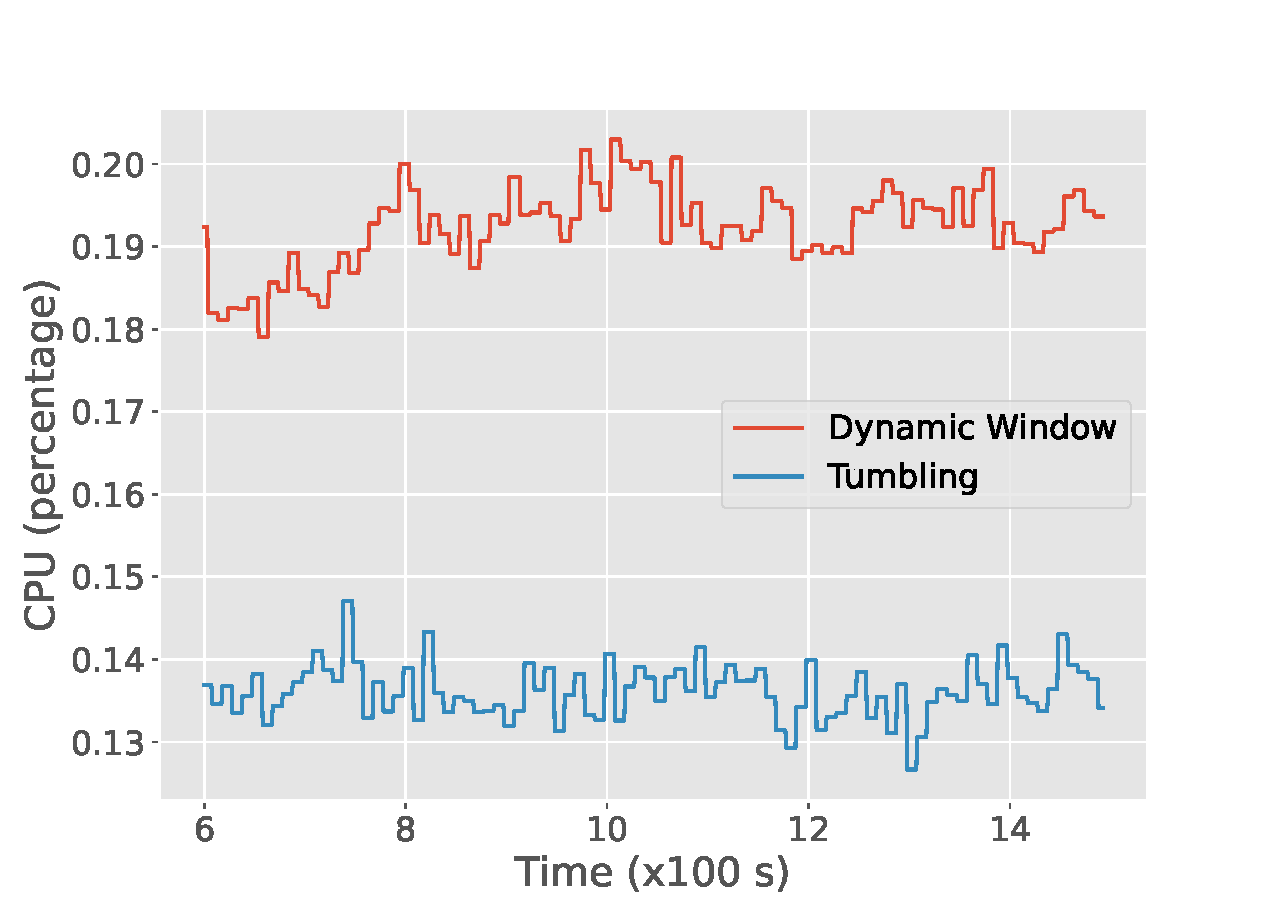
\includegraphics[width=\columnwidth]{fig/constant-rate/cpu_comparison.pdf}
        \caption{CPU-gebruik}
        \label{fig:constant_cpu}
    \end{subfigure}
    \begin{subfigure}[b]{0.5\columnwidth}
        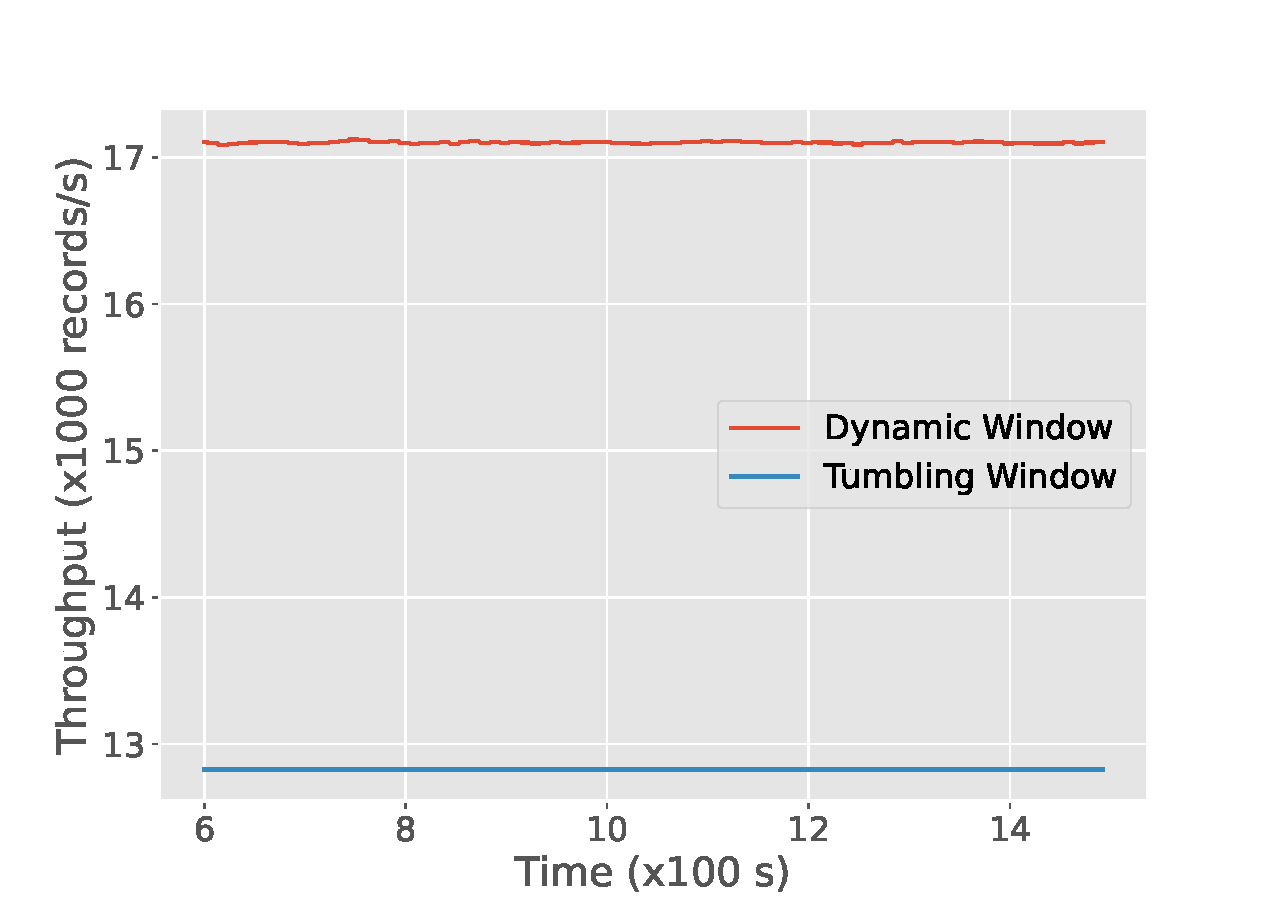
\includegraphics[width=\columnwidth]{fig/constant-rate/throughput_comparison.pdf}
        \caption{Doorvoer}
        \label{fig:constant_thorughput}
    \end{subfigure}
    %%
    \\
    \begin{subfigure}[b]{0.5\columnwidth}
        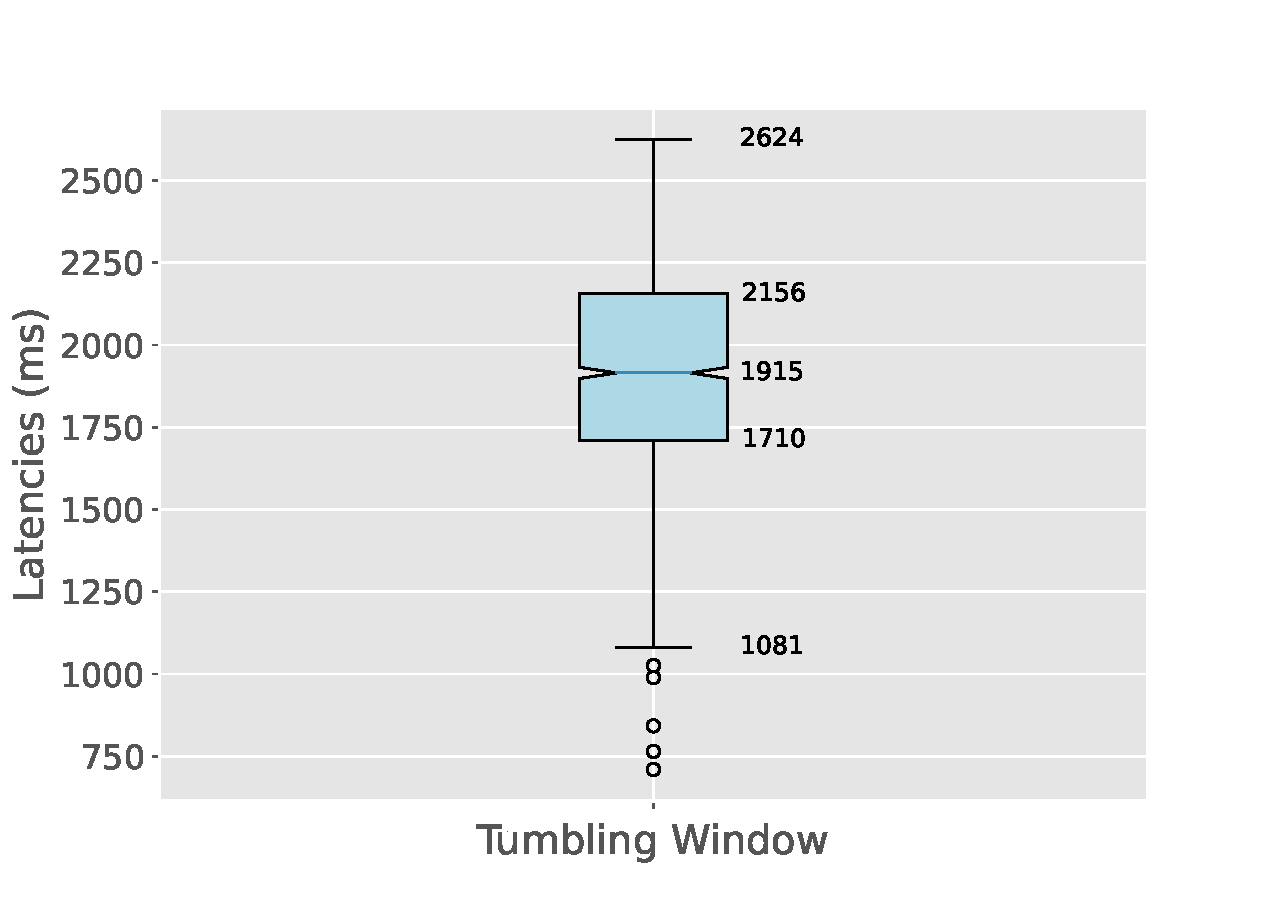
\includegraphics[width=\columnwidth]{fig/constant-rate/TumblingWindow_latency_boxplot.pdf}
        \caption{Tumbling latency}
        \label{fig:constant_tumb_boxplot}
    \end{subfigure}
    \begin{subfigure}[b]{0.5\columnwidth}
        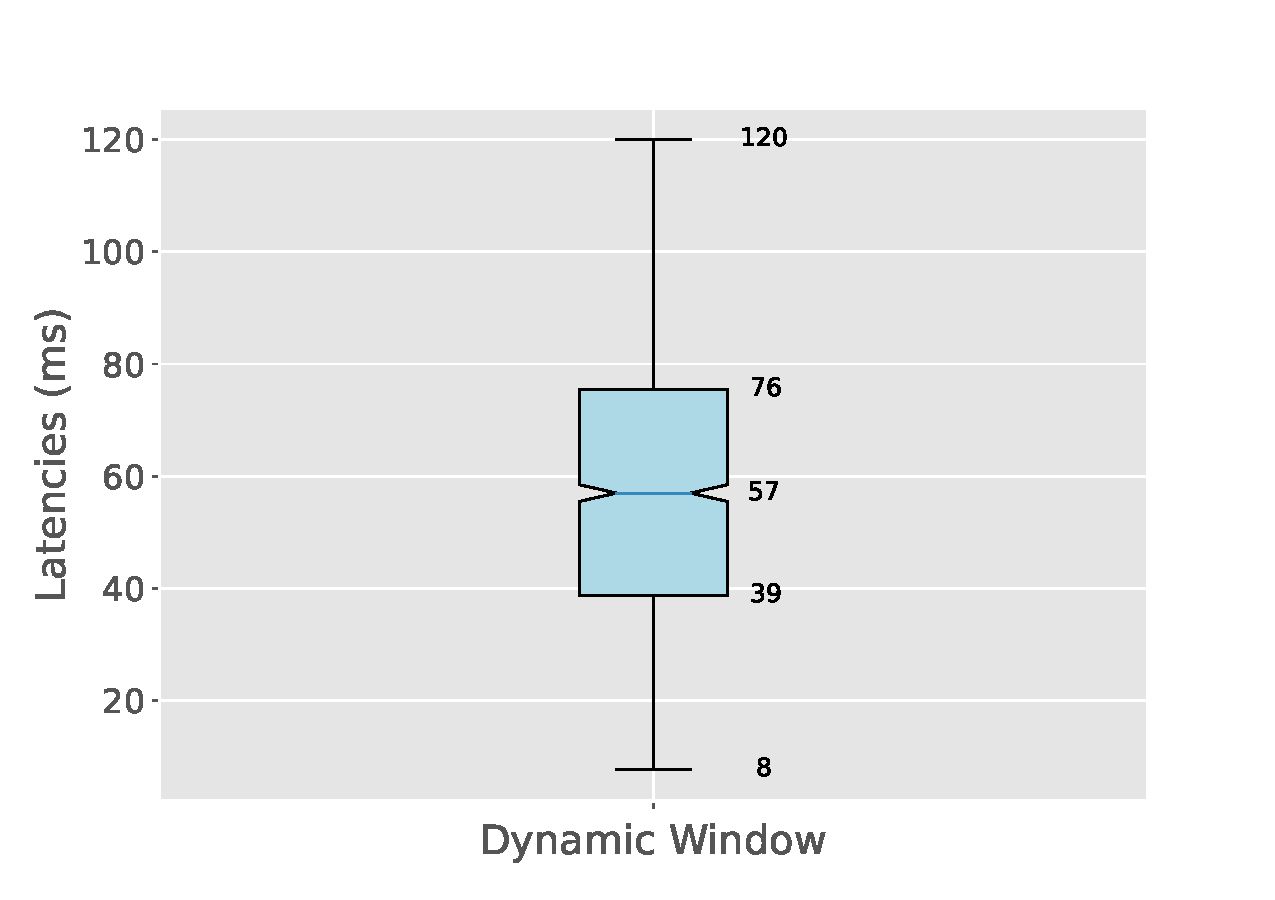
\includegraphics[width=\columnwidth]{fig/constant-rate/DynamicWindow_latency_boxplot.pdf}
        \caption{Dynamische latentie}
        \label{fig:constant_dynamic_boxplot}
    \end{subfigure}
    % \\
    \\
    \begin{subfigure}[b]{\columnwidth}
        \centering
        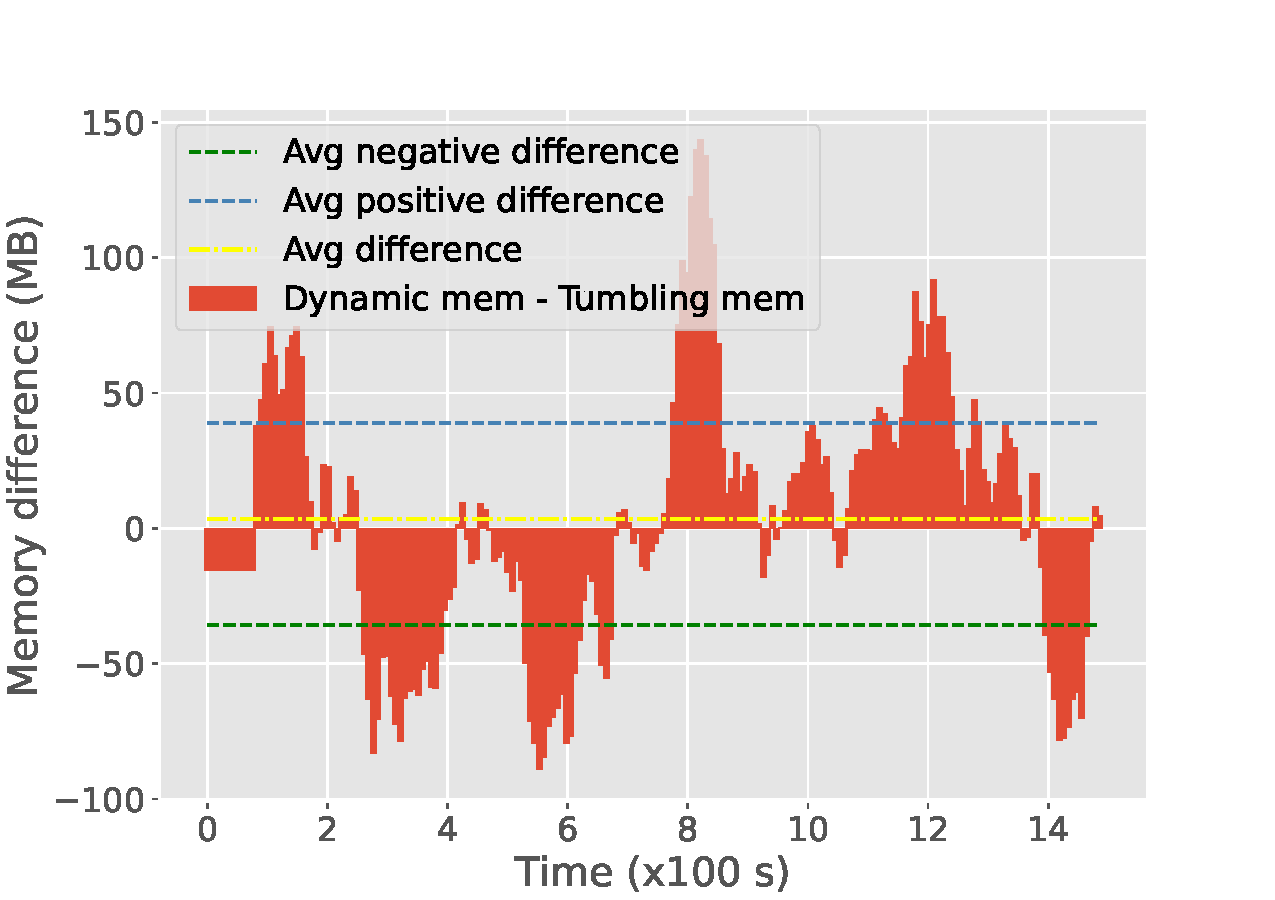
\includegraphics[width=0.5\columnwidth]{fig/constant-rate/mem_difference_bar.pdf}
        \caption{Relatief verschil in geheugengebruik vanuit het oogpunt van een dynamisch venster}
        \label{fig:constant_mem_diff}
    \end{subfigure}

    \caption[Metriek metingen voor latency werklast.]
    {Metingen voor latentie werklast. Dynamisch venster presteert 
    beter in alle metingen met uitzondering van CPU-gebruik als gevolg van
overhead in dynamische aanpassing van subvenster maten.}%
    \label{fig:constant_measurement}
\end{figure}

\subsection{Werklast voor periodieke burst}%
\label{sec:Results Workload for periodic burst}

Dynamisch venster verwerkt nog steeds de periodieke burst van gegevens met lagere latency 
dan Tumbling venster met latency in het bereik van 8ms tot 1669ms
(Figuur ~\ref{fig:periodic_dynamic_boxplot}) vergeleken met 
Tumbling venster's bereik van 891 ms tot 3904 ms 
(Figuur ~\ref{fig:periodic_tumb_boxplot}) die het dubbele is van de latentie 
gemeten voor Dynamisch venster.
Er is echter een tijdelijke toename in latentie aan het begin 
(Figuur ~\ref{fig:periodic_dynamic_lineplot}), 
wanneer de gegevensstoot elke 10e seconde arriveert. 
Dit is te wijten aan de aanvankelijke grootte van 2s subvensters voor de aanvankelijk lage streamsnelheid van 400 records per seconde. 
De grootte van de subvensters begint \textbf groter te worden dan 2s vanwege de lage stroomsnelheid. 
De toename in de subvenster grootte resulteert in het 
venster meer records te verwerken krijgt, waardoor tegendruk ontstaat en de latentie toeneemt.  
Dit resulteert in een positieve scheefheid in de latentiedistributie voor Dynamisch venster (figuur ~\ref{fig:periodic_dynamic_boxplot}). 
Dynamisch venster slaagt er echter uiteindelijk in de subwindow-groottes te verkorten als een
aan te passen aan de periodieke uitbarsting van gegevens tot het weer een latentietijd van minder dan een seconde bereikt.


De doorvoer van beide vensters steeg zoals verwacht.
Bovendien zien we een groter verschil in de doorvoer tussen de 
twee vensters van ongeveer 6000 records per seconde 
(figuur~\ref{fig:periodic_throughput}). Echter, de
constante en vlakke doorvoermeting stemt echter niet overeen 
met de resultaten van ~\cite{evalution_of_spe} waar er duidelijke "pieken" zijn in 
de doorvoermeting die overeenkomen met de periodieke uitbarsting 
van records die door de vensters worden verwerkt. 
We voerden onze evaluatie uit als onderdeel van de gehele RMLStreamer pijplijn, waardoor 
een lichte tegendruk 
wat leidt tot een hoge en vlakke doorvoermeting. 


CPU gebruik verschil van de vensters, is vergelijkbaar met de 
werklast voor latentiemeting met relatieve toename voor 
burst data verwerking
(Figuur ~\ref{fig:periodic_cpu}). 

Verrassend,
gebruikt het dynamische venster 
gemiddeld ongeveer 10 MB minder geheugen dan het Tumbling-venster gedurende de evaluatieperiode 
(Figuur ~\ref{fig:periodic_mem_diff}). 
Het aanvankelijke geheugengebruik voor Dynamisch venster is ongeveer 100 MB hoger dan voor 
Tumbling venster als gevolg van de lange groei van het venster 
veroorzaakt door de lage streamsnelheid. Echter, zodra 
de dynamische aanpassing van subwindow in werking treedt, wordt het geheugengebruik verminderd.


\begin{figure}
    \begin{subfigure}[b]{\columnwidth}
        \centering
        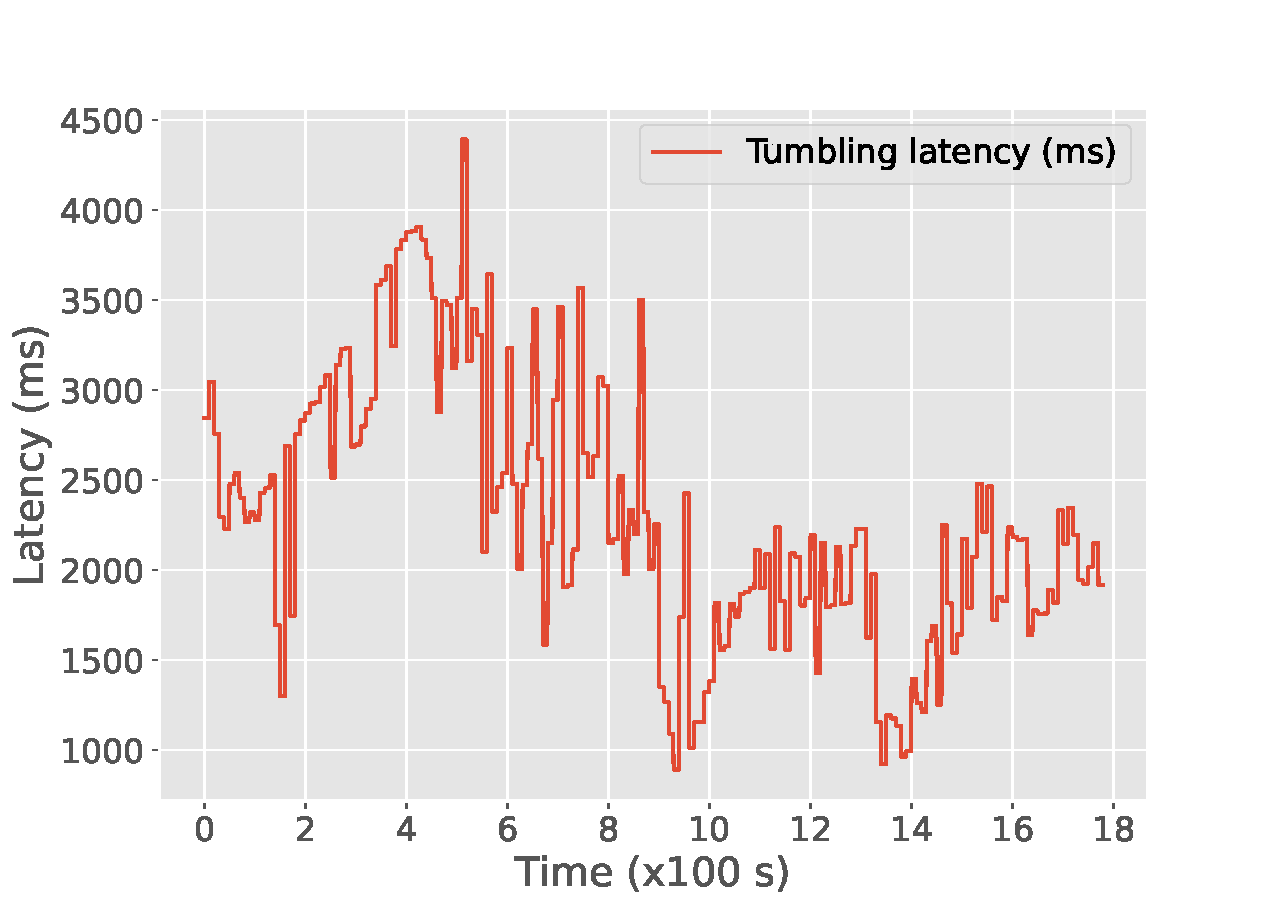
\includegraphics[width=0.8\columnwidth]{fig/periodic/Tumbling_latency_lineplot.pdf}
        \caption{Tumbling latency }
        \label{fig:periodic_tumbling_lineplot}
    \end{subfigure}

    \begin{subfigure}[b]{\columnwidth}
        \centering
        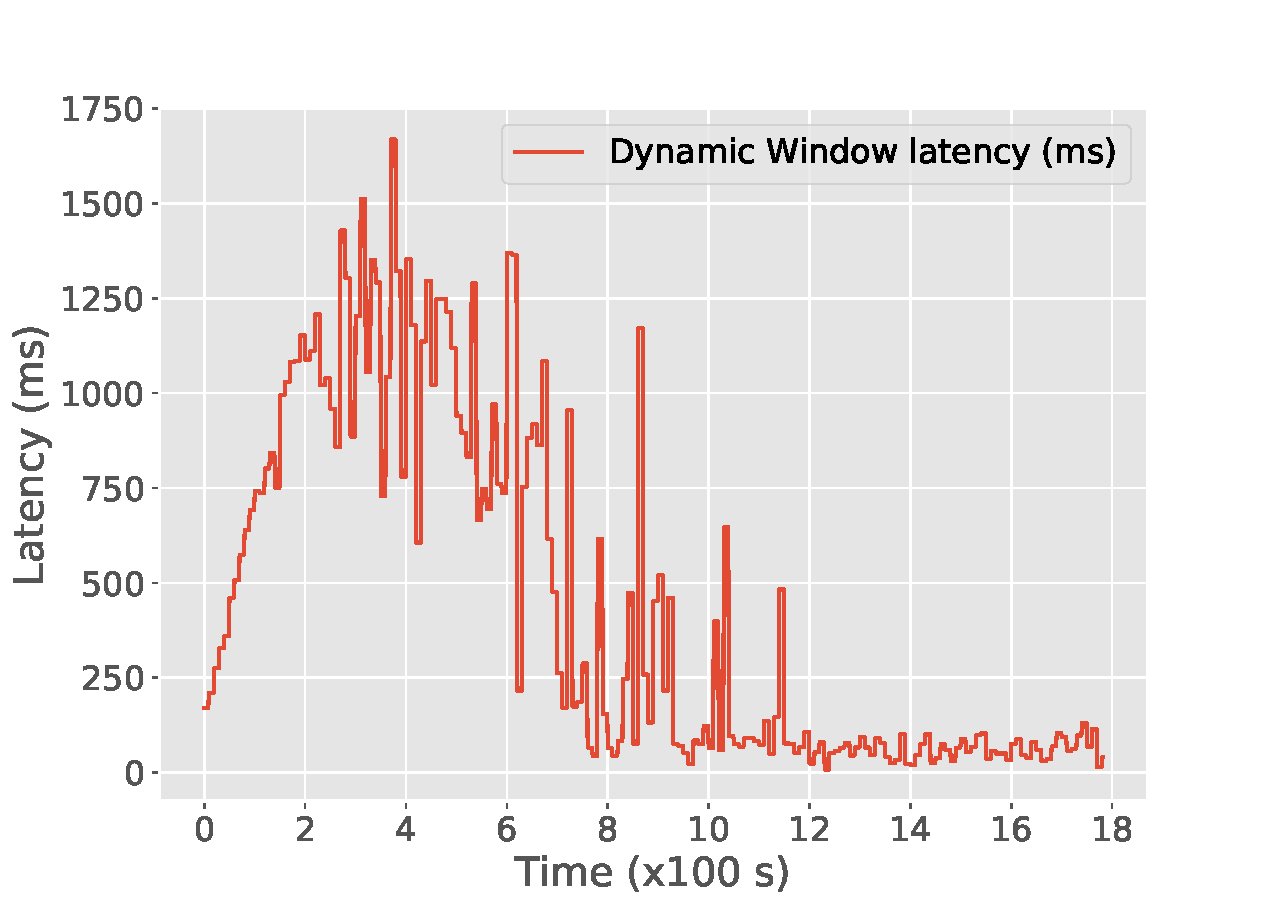
\includegraphics[width=0.8\columnwidth]{fig/periodic/DynamicWindow_latency_lineplot.pdf}
        \caption{Dynamische latentie }
        \label{fig:periodic_dynamic_lineplot}
    \end{subfigure}
    \caption{Latency meting van periodieke werklast gedurende de evaluatieperiode}
    \label{fig:periodic_latency_lineplot}
\end{figure}

\begin{figure}
    \begin{subfigure}[b]{0.5\columnwidth}
        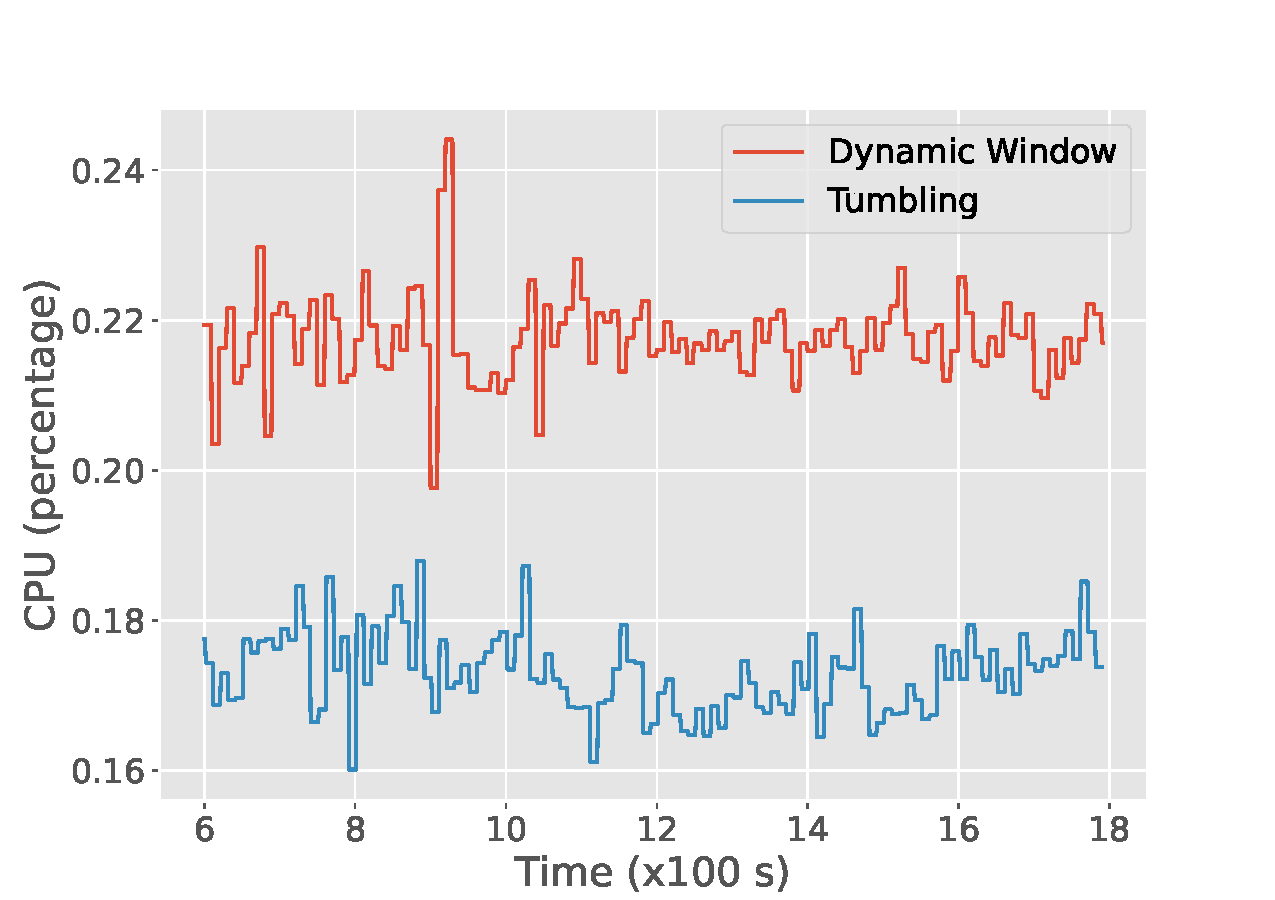
\includegraphics[width=\columnwidth]{fig/periodic/cpu_comparison.pdf}
        \caption{CPU gebruik}
        \label{fig:periodic_cpu}
    \end{subfigure}
    \hfill 
    \begin{subfigure}[b]{0.5\columnwidth}
        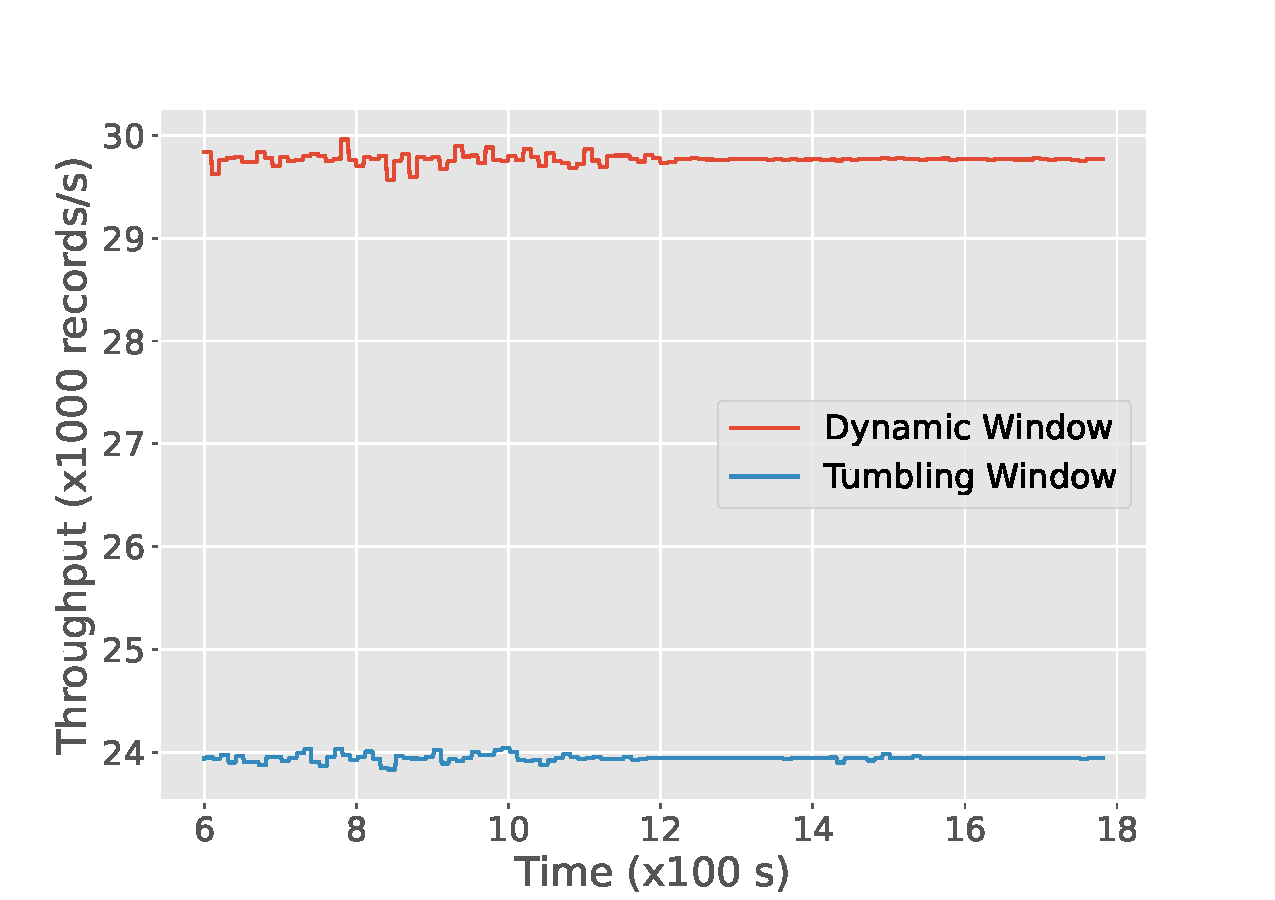
\includegraphics[width=\columnwidth]{fig/periodic/throughput_comparison.pdf}
        \caption{Doorvoer}
        \label{fig:periodic_throughput}
    \end{subfigure}
    %%
    \begin{subfigure}[b]{0.5\columnwidth}
        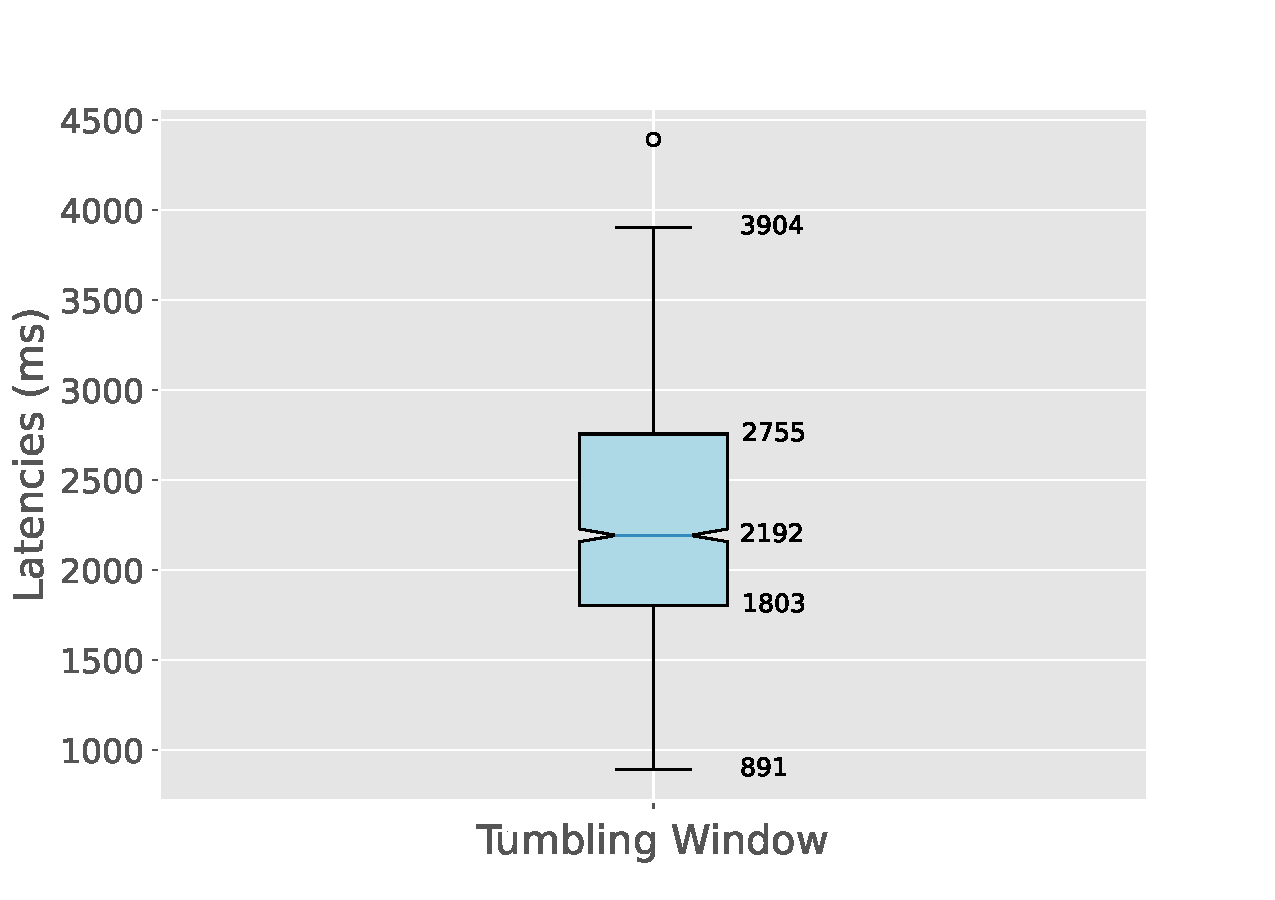
\includegraphics[width=\columnwidth]{fig/periodic/TumblingWindow_latency_boxplot.pdf}
        \caption{Tumbling latency distribution}
        \label{fig:periodic_tumb_boxplot}
    \end{subfigure}
    \hfill 
    \begin{subfigure}[b]{0.5\columnwidth}
        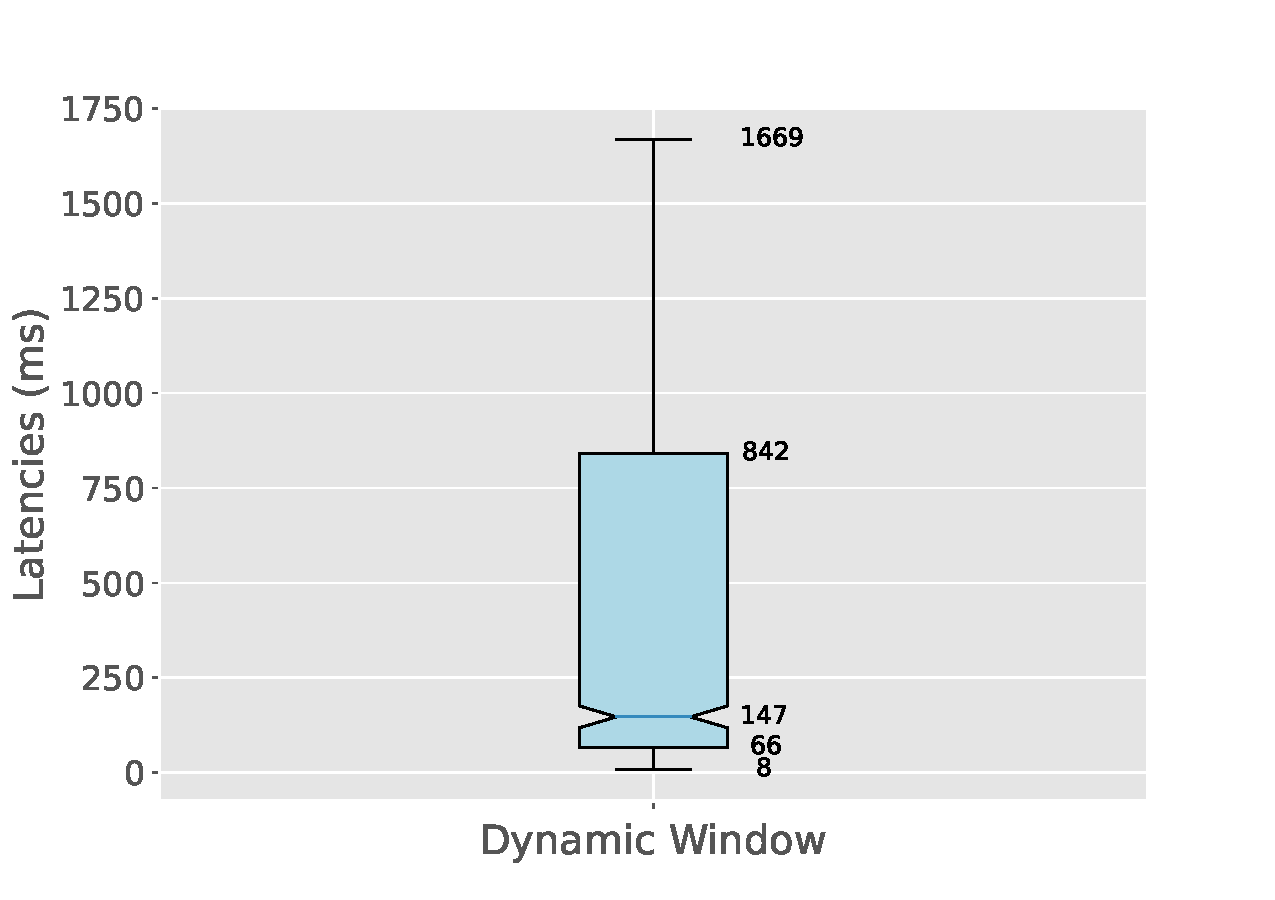
\includegraphics[width=\columnwidth]{fig/periodic/DynamicWindow_latency_boxplot.pdf}
        \caption{Dynamische latentiedistributie}
        \label{fig:periodic_dynamic_boxplot}
    \end{subfigure}
    % 
    \begin{subfigure}[b]{\columnwidth}
        \centering
        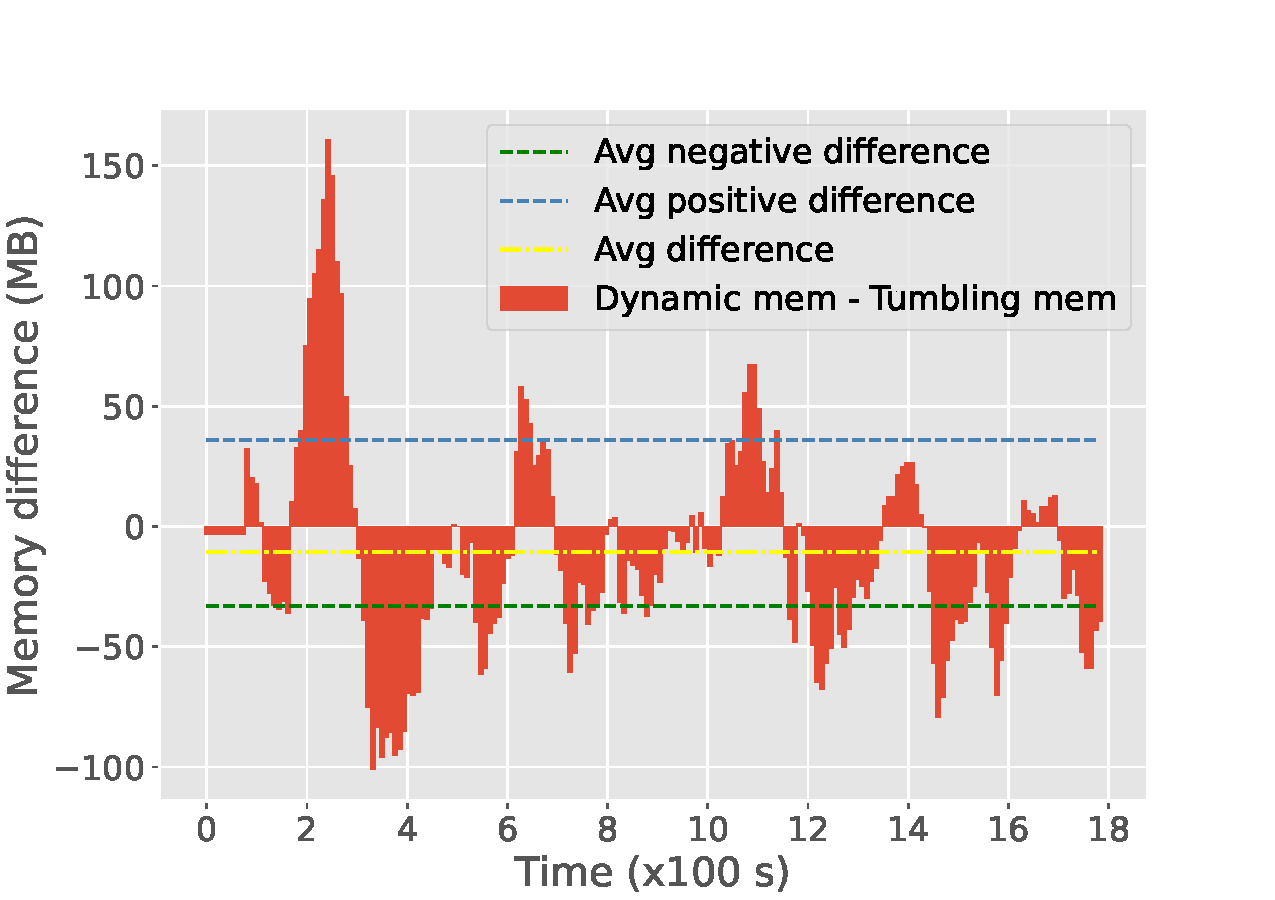
\includegraphics[width=0.5\columnwidth]{fig/periodic/mem_difference_bar.pdf}
        \caption{Relatief verschil in geheugengebruik vanuit het oogpunt van dynamisch venster}
        \label{fig:periodic_mem_diff}
    \end{subfigure}

    \caption[Metriek metingen voor periodieke werklast]
    {Metrics metingen voor periodieke werklast. Dynamisch venster 
    heeft gemiddeld lager geheugengebruik dan Tumbling venster voor
periodieke werklast. }%
    \label{fig:periodic_measurement}
\end{figure}

\subsection{Werklast voor volledigheidsmeting}%
\label{sec:Workload for completeness measure}

Uit de resultaten in tabel~\ref{tab:dynamic_completeness}, en 
Tabel ~\ref{tab:tumbling_completeness}, concluderen we dat Dynamisch venster 
beter presteert dan Tumbling venster wat betreft het genereren van een meer \emph{complete} output. 
Dynamisch venster heeft een IOU score van \textbf{1} voor constante lage stream rate
doordat de subwindow groot genoeg wordt 
groot genoeg worden om alle vereiste records te bevatten, om de \emph{complete} output set te genereren. Daarentegen scoort het Tumbling venster slechts \textbf{0.749}, wat leidt tot 
de conclusie dat een venstergrootte van 2s niet genoeg is om de lage stroomsnelheid 
van de evaluatiegegevens. 

Ook voor periodieke burst-invoer presteert Dynamic window beter dan Tumbling venster met een
score van \textbf{0.982}, terwijl Tumbling venster slechts \textbf{0.780} scoort. De hoge IOU 
score van Dynamisch venster is te danken aan zijn vermogen  
om zich aan te passen aan de veranderende stroomsnelheid om genoeg 
records vast te houden voor maximale gezamenlijke output generatie.


\begin{table}[htbp]
    \centering
    \resizebox{0.5\columnwidth}{!}{%
\begin{tabular}{|r|r|}
\hline
\multicolumn{1}{|c|}{Stream rate} & \multicolumn{1}{c|}{\textbf{IOU score}} \\ \hline
Constante snelheid & \textbf{1} \\ \hline
Periodieke uitbarsting & \textbf{0.982}                          \\ \hline
\end{tabular}%
}
\caption{Dynamisch venster meting van volledigheid.}
\label{tab:dynamic_completeness}
\end{table}

\begin{table}[htbp]
    \centering
    \resizebox{0.5\columnwidth}{!}{%
\begin{tabular}{|r|r|}
\hline
\multicolumn{1}{|c|}{Stream rate} & \multicolumn{1}{c|}{\textbf{IOU score}}\\ \hline
Constante koers & \textbf{0.749}                              \\ \hline
Periodieke uitbarsting & \textbf{0.780}                          \\ \hline
\end{tabular}%
}
\caption{Tumbling venster meting van volledigheid. }
\label{tab:tumbling_completeness}
\end{table}


\subsection{Samenvatting}
\label{sec:Result Summary}

Samenvattend, tonen deze resultaten aan dat onze implementatie van Dynamisch venster 
lagere latency, hogere doorvoer, en een meer complete 
uitvoer dan Tumbling venster voor zowel 
werklasten van constante stream rate, en onstabiele periodieke burst stream rate.

Hoewel het geheugengebruik daalde in de werklast met periodieke burst snelheid, konden we 
konden we niet met zekerheid concluderen dat het Dynamisch venster effectief minder geheugen gebruikte
dan het Tumbling venster. De meting was gebaseerd op het heap geheugen van de 
hele evaluatie job, niet alleen van de window operator. Daarom is er behoefte aan een 
nauwkeurigere meting van het geheugengebruik. 

De resultaten voor doorvoer wijken ook af van die van Van Dongen en Van den Poel(2020)~\cite{evalution_of_spe}. 
Dit is te wijten aan het feit dat we de evaluatie hebben uitgevoerd met de volledige pijplijn van RMLStreamer. Hierdoor ontstaat enige tegendruk van de mapping stage, 
waardoor de doorvoer van de join-fase constant en vlak blijft.    

Over het geheel genomen kunnen we concluderen dat Dynamic windowing een goed alternatief is voor de vaste 
vensters. Vooral in gebruik 
gevallen, waar vensters niet van vaste grootte hoeven te zijn met een variabele stroomsnelheid.  


\section{Conclusion and Future Works}%
\label{chap:Conclusion and Future Works}

In this paper, we have presented an approach for Dynamic window 
which adapts its window size according to the stream rate of the 
input data sources. We introduced a simple heuristic to adapt 
window sizes dynamically without huge memory or computation overhead. 

We implemented our Dynamic window on top of the existing RMLStreamer, 
to evaluate its performance under a realistic processing environment. 
We adapted the benchmark framework as stated in~\cite{evalution_of_spe} to 
accurately evaluate the performance of our implementation against the 
standard fixed size Tumbling window. 

The results show that our implementation 
of Dynamic window performs better than Tumbling window in terms of 
latency, throughput, and completeness with only a slight 
increase in CPU usage. Even though we could not confidently conclude that
memory usage is lower in Dynamic window, our preliminary results indicate 
that it performs the same as Tumbling window in the worst-case scenario.

Therefore, there are still areas of improvement to be made.
On the evaluation side, we could further increase 
the precision of our memory measurement by only counting the number of records
residing in the windows at any moment instead of the whole JVM heap of the RMLStreamer job. 
Furthermore, the evaluation could be done in the same benchmark pipelines as in~\cite{evalution_of_spe} 
to further evaluate the Dynamic window performance in a general stream processing case.
Improvements on our dynamic approach could be achieved by allowing users to 
define other statistical approaches
to better calculate the threshold for adapting the window sizes. 



%%%%%%%%%%%%%%%%%%%%%%%%%%%%%%%%%%%%%%%%%%%%%%%%%%%%%%%%%%%%%%%%%%%%%%%%%%%%%%%%

\printbibliography

\end{document}
